\documentclass[a4paper,11pt]{article}

\usepackage[utf8]{inputenc}

\usepackage{minted}
\usepackage{graphicx}

\begin{document}


\title{
    \textbf{Doubly report}
}
\author{Jonathan Karlsson}
\date{Fall 2023}

\maketitle

\section*{Introduction}
This assignment was to create a double linked list and compare it to a single linked list when inserting and unlinking.


\section*{Implementation}
For the assignment the same four basic methods add, length, find and remove had to be added but for a double linked list. 
The first method add was changed so that when adding an item as first, the original first got a prev reference to the new first.
\begin{minted}{java}
public void add(int item) {
    Cell firstcopy = this.first;
    this.first = new Cell(item, this.first,null);
    if (firstcopy != null)
        firstcopy.prev = first;
}    
\end{minted}
The second method length was not changed from the single linked list as it only uses next and goes through the list. 
The same thing is true with the find which also only goes through the list using next. 
\newline
\newline
The final method remove had to be rewritten as it has to remove the reference to prev from the cell that it removes aswell. 
The new remove method works by going through every cell in the list, and if the head is the same as item 3 different scenarios can occur. 
The first is if both prev and next is not null, which means that the element was somewhere in the middle of the list. Then the next reference of the prevoius cell is set to the next reference of the current cell and
the prev reference of the next cell is set as the prev reference of the current cell. 
The second scenario is if the next cell is null, this means that the cell is at the end of the list and the only thing that has to be done is change the next reference of the prevoius cell to null, to turn the prevoius cell into 
the last cell of the list. 
The final scenario is if no of the other two statements were true, which means that the cell is the first cell of the list. To remove the cell the first of the list is changed to the next cell and the prev of the new first is set to null, 
so that it is actually the first cell.

\begin{minted}{java}
public void remove(int item) {
    Cell next = this.first;
    while (next != null){
        if (next.head == item){
            if (next.prev != null && next.next != null){
                next.prev.next = next.next;
                next.next.prev = next.prev;
                }
            else if(next.next == null) {
                next.prev.next = null;
            }
            else{
                this.first = next.next;
                this.first.prev = null;   
            }
            break;
        }
        next = next.next;
    }
}    
\end{minted}
\noindent
There were also two methods unlink and insert, which had to be made for both double linked list and single linked list. 
For the double linked list, the unlink method uses the same three if statements as the remove but with the cell that was given to it instead of a cell that was found,
this works because the cell that is given to it is the same as the cell in the list, which means if it is changed, the cell in the list is also changed. This makes it easy to change the 
double linked list, as each cell knows the cell before itself and the cell after itself, which makes it possible to only know a cell to remove it, it is not necessary to find it in the list.
\begin{minted}{java}
public void unlink(Cell cell) {
    if (cell.prev != null && cell.next != null) {
        cell.prev.next = cell.next;
        cell.next.prev = cell.prev;
    }
    else if(cell.next == null) {
        cell.prev.next = null;
    }
    else {
        this.first = cell.next;
        this.first.prev = null;   
    }  
}    
\end{minted}
The unlink for the single linked list is more difficult, as it is impossible to know which cell comes before the cell that should be removed. This means that 
it is first required to go through the list while keeping track of next and prev, and then when the cell in the list is the same as the cell searched for, if prev is not null, which means the cell is in the middle of the list, 
remove it by setting prev.tail to next.tail. If prev was null it was the first cell, so set the first cell as the cell after the first cell.
\begin{minted}{java}
public void unlink(CellSingle cell) {
    CellSingle next = this.first;
    CellSingle prev = null;
    while (next != null) {
        if (next.equals(cell)) {
            if (prev != null)
                prev.tail = next.tail;
            else
                this.first = next.tail;
            break;
        }  
        prev = next;
        next = next.tail;   
    }
}
\end{minted}
The insert methods are very simple for both the single and double linked list. For the double linked list it works by first checking if the first is not null, as that would mean that it is not possible to set the prev of the first. If first was not null it sets 
prev of first to be the cell that will be inserted. Then the cell.next is set to first, it does not matter if first is null here as if it is, it would only mean that the cell is the only cell in the list.
Then the first is set to cell, and finally the first, which is now the inserted cell, has its prev set to null. Setting the cells prev to null is something that depends on the usecase, as sometimes the cell might 
be used somewhere else aswell, then it would be bad to set its prev to null, but as it will only be used in one list in this assignment it gets set to null here to indicate the start of the list. Otherwise, the list might get infinite if the cell prevoiusly 
was at a position inside the list, which would mean its prev still would be pointing there. 
\begin{minted}{java}
public void insert(Cell cell) {
    if(this.first!= null)
        this.first.prev = cell;
    cell.next = this.first;
    this.first = cell;
    this.first.prev = null; //maybe not neccesary, depends on function.
}
\end{minted}
The insert for the single linked list only sets the tail of the new cell to first and then sets the cell as first.
\begin{minted}{java}
public void insert(CellSingle cell) {
    cell.tail = this.first;
    this.first = cell;
}
\end{minted}
\section*{Benchmark}
The Benchmark for this assignment was to compare unlinking and then inserting 1000 random cells, from n size single and double linked lists. 
The data from the two different linked lists can be found in the table below.
\begin{table}[h]
    \begin{center}
    \scalebox{0.8}{
    \begin{tabular}{l|c|c|}
    \textbf{n} & \textbf{Double linked list({\textmu}s)} & \textbf{Single linked list({\textmu}s)}\\
    \hline
    1000     &  6 &     550 \\
    1100     &  6 &     660 \\
    1200     &  6 &     710 \\
    1300     &  6 &     770 \\
    1400     &  6 &     770 \\
    1500     &  6 &     860 \\
    1600     &  6 &     910 \\
    3200     &  6 &    1800 \\
    6400     &  6 &    2300 \\
   12800     &  8 &    3000 \\
   25600     &  9 &    4000 \\
   51200     & 13 &    4700 \\
  102400     & 17 &    4800 \\
  204800     & 45 &    5000 \\

    \end{tabular}
    }
    \caption{The result of using unlink and insert on the two lists}
    \label{tab:table1}
    \end{center}
\end{table}
{\noindent}
\newline
As most of the insert methods are the same, it is safe to assume that the reason that the single linked list takes so much longer than the double linked list 
is because of the unlink method, which also makes sense as the single linked list has to go through every cell until it finds the cell that should be unlinked and then unlinks it. This should 
theoretically be of $O(n)$. The double linked list however does not need to go through the list to remove a cell from it, therefore it should theoretically be constant time or $O(1)$. This can also
be seen in the table, however it seems to slow down a bit when n gets larger, this is probably because it takes longer time to look up the specific cell in the memory, when there are more data in the memory.
\newline
\newline
When looking at a graph of the two linked lists it is possible to see that the single linked list starts linear, but then the change of time depending on n slows down
so it gets more constant, this can also be seen in the table as the nnumber of elements double but the time only increases with 1.05 times. This might depend on how "lucky" the method got when looking for the cell, if the cell is in the beginning
the method is obviously faster than if it is in the end
\begin{figure}[h]
    \centering    
    
    \scalebox{0.8}{% GNUPLOT: LaTeX picture with Postscript
\begingroup
  \makeatletter
  \providecommand\color[2][]{%
    \GenericError{(gnuplot) \space\space\space\@spaces}{%
      Package color not loaded in conjunction with
      terminal option `colourtext'%
    }{See the gnuplot documentation for explanation.%
    }{Either use 'blacktext' in gnuplot or load the package
      color.sty in LaTeX.}%
    \renewcommand\color[2][]{}%
  }%
  \providecommand\includegraphics[2][]{%
    \GenericError{(gnuplot) \space\space\space\@spaces}{%
      Package graphicx or graphics not loaded%
    }{See the gnuplot documentation for explanation.%
    }{The gnuplot epslatex terminal needs graphicx.sty or graphics.sty.}%
    \renewcommand\includegraphics[2][]{}%
  }%
  \providecommand\rotatebox[2]{#2}%
  \@ifundefined{ifGPcolor}{%
    \newif\ifGPcolor
    \GPcolortrue
  }{}%
  \@ifundefined{ifGPblacktext}{%
    \newif\ifGPblacktext
    \GPblacktextfalse
  }{}%
  % define a \g@addto@macro without @ in the name:
  \let\gplgaddtomacro\g@addto@macro
  % define empty templates for all commands taking text:
  \gdef\gplbacktext{}%
  \gdef\gplfronttext{}%
  \makeatother
  \ifGPblacktext
    % no textcolor at all
    \def\colorrgb#1{}%
    \def\colorgray#1{}%
  \else
    % gray or color?
    \ifGPcolor
      \def\colorrgb#1{\color[rgb]{#1}}%
      \def\colorgray#1{\color[gray]{#1}}%
      \expandafter\def\csname LTw\endcsname{\color{white}}%
      \expandafter\def\csname LTb\endcsname{\color{black}}%
      \expandafter\def\csname LTa\endcsname{\color{black}}%
      \expandafter\def\csname LT0\endcsname{\color[rgb]{1,0,0}}%
      \expandafter\def\csname LT1\endcsname{\color[rgb]{0,1,0}}%
      \expandafter\def\csname LT2\endcsname{\color[rgb]{0,0,1}}%
      \expandafter\def\csname LT3\endcsname{\color[rgb]{1,0,1}}%
      \expandafter\def\csname LT4\endcsname{\color[rgb]{0,1,1}}%
      \expandafter\def\csname LT5\endcsname{\color[rgb]{1,1,0}}%
      \expandafter\def\csname LT6\endcsname{\color[rgb]{0,0,0}}%
      \expandafter\def\csname LT7\endcsname{\color[rgb]{1,0.3,0}}%
      \expandafter\def\csname LT8\endcsname{\color[rgb]{0.5,0.5,0.5}}%
    \else
      % gray
      \def\colorrgb#1{\color{black}}%
      \def\colorgray#1{\color[gray]{#1}}%
      \expandafter\def\csname LTw\endcsname{\color{white}}%
      \expandafter\def\csname LTb\endcsname{\color{black}}%
      \expandafter\def\csname LTa\endcsname{\color{black}}%
      \expandafter\def\csname LT0\endcsname{\color{black}}%
      \expandafter\def\csname LT1\endcsname{\color{black}}%
      \expandafter\def\csname LT2\endcsname{\color{black}}%
      \expandafter\def\csname LT3\endcsname{\color{black}}%
      \expandafter\def\csname LT4\endcsname{\color{black}}%
      \expandafter\def\csname LT5\endcsname{\color{black}}%
      \expandafter\def\csname LT6\endcsname{\color{black}}%
      \expandafter\def\csname LT7\endcsname{\color{black}}%
      \expandafter\def\csname LT8\endcsname{\color{black}}%
    \fi
  \fi
    \setlength{\unitlength}{0.0500bp}%
    \ifx\gptboxheight\undefined%
      \newlength{\gptboxheight}%
      \newlength{\gptboxwidth}%
      \newsavebox{\gptboxtext}%
    \fi%
    \setlength{\fboxrule}{0.5pt}%
    \setlength{\fboxsep}{1pt}%
    \definecolor{tbcol}{rgb}{1,1,1}%
\begin{picture}(7200.00,5040.00)%
    \gplgaddtomacro\gplbacktext{%
      \csname LTb\endcsname%%
      \put(1210,704){\makebox(0,0)[r]{\strut{}$1$}}%
      \put(1210,1390){\makebox(0,0)[r]{\strut{}$10$}}%
      \put(1210,2076){\makebox(0,0)[r]{\strut{}$100$}}%
      \put(1210,2762){\makebox(0,0)[r]{\strut{}$1000$}}%
      \put(1210,3447){\makebox(0,0)[r]{\strut{}$10000$}}%
      \put(1210,4133){\makebox(0,0)[r]{\strut{}$100000$}}%
      \put(1210,4819){\makebox(0,0)[r]{\strut{}$1\times10^{6}$}}%
      \put(1890,484){\makebox(0,0){\strut{}$1000$}}%
      \put(3710,484){\makebox(0,0){\strut{}$10000$}}%
      \put(5531,484){\makebox(0,0){\strut{}$100000$}}%
    }%
    \gplgaddtomacro\gplfronttext{%
      \csname LTb\endcsname%%
      \put(209,2761){\rotatebox{-270}{\makebox(0,0){\strut{}time in µs}}}%
      \put(4072,154){\makebox(0,0){\strut{}n}}%
      \csname LTb\endcsname%%
      \put(3850,4646){\makebox(0,0)[r]{\strut{}Double linked list}}%
      \csname LTb\endcsname%%
      \put(3850,4426){\makebox(0,0)[r]{\strut{}Single linked list}}%
      \csname LTb\endcsname%%
      \put(3850,4206){\makebox(0,0)[r]{\strut{}n}}%
    }%
    \gplbacktext
    \put(0,0){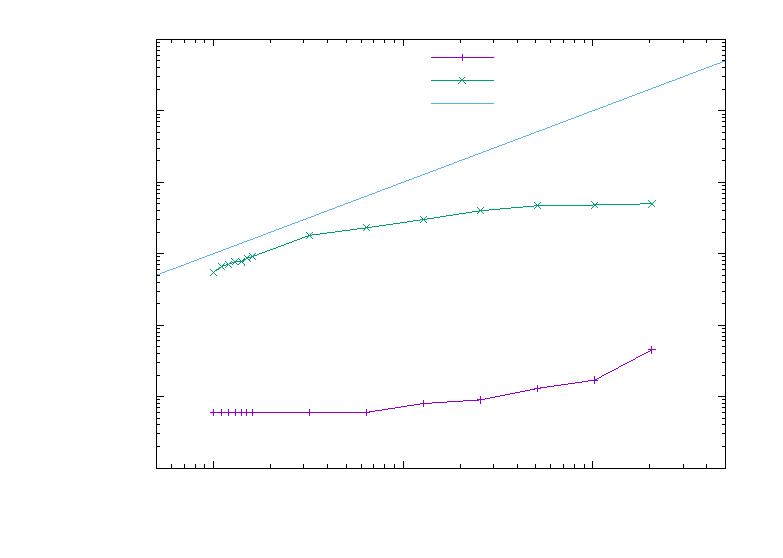
\includegraphics[width={360.00bp},height={252.00bp}]{disp}}%
    \gplfronttext
  \end{picture}%
\endgroup
}
    \caption{Visualization of using unlink and insert on the two lists}   
    \label{tab:figure1} 
    
    \end{figure}



\section*{Conclusion}
It seems that it is better to write double linked lists, as these are more flexible, even if some methods for the lists are a bit trickier to write, they are easier to work with, for example when using 
the unlink method as it is posslible to just remove a selected cell without knowing the rest of the list. It is also easier to navigate a double linked list, as it is always possible to go backwards without having
to save the prevoius cell separately.







\end{document}
